\documentclass[conference]{IEEEtran}

\usepackage{amsmath,amssymb}
\usepackage{mathtools}
\usepackage{algorithm}
\usepackage{algpseudocode}
\usepackage{graphicx}
\usepackage{booktabs}
\usepackage{multirow}
\usepackage{xcolor}
\usepackage{hyperref}
\usepackage{pgfplots}
\usepackage{tikz}
\usetikzlibrary{arrows.meta,positioning,shapes,fit,backgrounds}\pgfplotsset{compat=1.18}

\newcommand{\CEI}{\mathrm{CEI}}
\newcommand{\CRP}{\mathrm{CRP}}
\newcommand{\ABRS}{\mathrm{ABRS}}
\newcommand{\RV}{\mathrm{RV}}
\newcommand{\ALE}{\mathrm{ALE}}
\newcommand{\FAIR}{\mathrm{FAIR}}
\newcommand{\TEF}{\mathrm{TEF}}
\newcommand{\LM}{\mathrm{LM}}
\newcommand{\bx}{\mathbf{x}}
\newcommand{\E}{\mathbb{E}}
\newcommand{\Var}{\mathrm{Var}}
\newcommand{\logit}{\mathrm{logit}}
\DeclareMathOperator*{\argmax}{arg\,max}

\usepackage{listings}
\lstset{
    basicstyle=\ttfamily\footnotesize,
    breaklines=true,
    breakatwhitespace=true
}

\title{Continuous Compliance Monitoring with Real-Time Risk Quantification}
\author{
\IEEEauthorblockN{M. Caleb Gunalan}
\IEEEauthorblockA{
B.Tech Computer Science and Engineering\\
Kalasalingam Academy of Research and Education\\
Krishnankoil, Tamilnadu, India\\
calebgunalan2005@gmail.com
}
\and
\IEEEauthorblockN{Dr. P.~Deepalakshmi}
\IEEEauthorblockB{
Department of Computer Science and Engineering\\
Kalasalingam Academy of Research and Education\\
Krishnankoil, Tamilnadu, India\\
deepa.kumar@klu.ac.in
}
% \and
% \IEEEauthorblockN{~~~~~~~~~~~~Chinnasamy~Ponnusamy}
% \IEEEauthorblockC{
% ~~~~Department of Computer Science and Engineering\\
% ~~~~Kalasalingam Academy of Research and Education\\
% ~~~~~~~~~~~~Krishnankoil, Tamilnadu, India\\
% ~~~~~~~~~~~~chinnasamyponnusamy@gmail.com
% }
% \and
% \IEEEauthorblockN{~~~~~~~~~~~~Vidhya~Prakash~Rajendran}
% \IEEEauthorblockD{
% ~~~~~~~~~~~~Engineering Department\\
% ~~~~~~~~~~~~University of Technology and Applied Science\\ 
% ~~~~~~~~~~~~Nizwa, Sultanate of Oman\\
% ~~~~~~~~~~~~vidhya.rajendran@utas.edu.om
% }
}

\begin{document}
\maketitle

\begin{abstract}
Cybersecurity compliance frameworks generate abundant data but fail to quantify how control posture translates to financial risk. Traditional risk models (e.g.\ FAIR~\cite{Jones2005}) use static inputs and treat controls independently, ignoring continuous evidence streams and control dependencies. We introduce the Continuous Compliance Real-Time Risk Quantification (CC-RRQ) framework, which treats each automated control test as Bayesian evidence updating loss estimates. CC-RRQ includes five novel components: the \emph{Compliance Entropy Index} (CEI) applying Shannon entropy to measure compliance disorder; Cascade Risk Propagation (CRP), a directed-acyclic-graph algorithm for cascading control failures; Adaptive Bayesian Risk Scoring (ABRS), a Beta--Bernoulli model integrating FAIR with continuous evidence; Temporal Risk Velocity and Acceleration (TRVA) for risk trends; and an LLM-based anomaly detector (LLM-CAD) for subtle gaming patterns. We implement these in an open-source platform and evaluate on a 12-month study of 63 organizations. Results show strong negative correlation between maturity and breach rate ($r=-0.741$, $p<0.001$), median detection time falling from 87.4 days to 3.2 hours, and a 62.3\% average ALE reduction for organizations improving from maturity level~2 to~4. These findings provide large-scale evidence that continuous, quantified compliance governance yields measurable financial risk reduction.
\end{abstract}

\begin{IEEEkeywords}
cybersecurity governance; risk quantification; continuous compliance
  monitoring; Bayesian inference; information entropy; cascade failure; FAIR
methodology; control dependency graph; anomaly detection; maturity model
\end{IEEEkeywords}


\section{Introduction}
When a CISO requests budget approval, discussions often rely on qualitative claims (e.g.\ "our risk is high") rather than quantitative measures. Organizations collect vast compliance data (logs, tests, assessments) but lack a mathematical link between compliance posture and financial risk. The FAIR framework~\cite{Jones2005} expresses risk as annual loss expectancy (threat-event frequency $\times$ vulnerability probability $\times$ loss magnitude), but in practice uses static parameters and assumes control independence, ignoring dependencies. Meanwhile, modern compliance tools (AWS Security Hub, Azure Policy, OpenSCAP, etc.) can rapidly check hundreds of controls, but only report pass/fail and do not quantify risk or learn from streaming data.

This paper bridges these approaches. We treat each automated control test as evidence (a Bernoulli observation) about attack likelihood, capture compliance disorder with information entropy, model failure propagation via control dependency graphs, and track risk trajectory derivatives for executives. Our contributions are:
\begin{enumerate}
  \item \textbf{Compliance Entropy Index (CEI):} First use of Shannon entropy to measure compliance posture disorder (Section~\ref{sec:cei}).
  \item \textbf{Cascade Risk Propagation (CRP):} A DAG algorithm computing downstream failure probability when upstream controls degrade (Section~\ref{sec:crp}).
  \item \textbf{Adaptive Bayesian Risk Scoring (ABRS):} A Beta--Bernoulli model fusing FAIR with continuous control-test evidence (Section~\ref{sec:abrs}).
  \item \textbf{Temporal Risk Velocity and Acceleration (TRVA):} A calculus-based model for monitoring risk trajectory (Section~\ref{sec:trva}).
  \item \textbf{LLM-Augmented Compliance Anomaly Detection (LLM-CAD):} A language-model pipeline for detecting compliance gaming patterns (Section~\ref{sec:llmcad}).
\end{enumerate}
Section~\ref{sec:related} reviews related work. Section~\ref{sec:framework} presents the CC-RRQ architecture. Sections~\ref{sec:cei}--\ref{sec:llmcad} introduce each algorithm. Section~\ref{sec:experiments} describes our empirical study. Section~\ref{sec:discussion} discusses results and limitations, and Section~\ref{sec:conclusion} concludes.

\section{Related Work}
\label{sec:related}

\subsection{Risk Quantification}
Cybersecurity risk quantification builds on actuarial and probabilistic analysis. The FAIR framework~\cite{Jones2005} formalizes risk as annual loss expectancy (ALE = threat-event frequency $\times$ vulnerability probability $\times$ loss magnitude, Eq.~\ref{eq:fair_basic}). Enhancements include Monte Carlo propagation~\cite{Hubbard2016}, multivariate loss models~\cite{Biener2015}, and Bayesian networks~\cite{Fielder2016,Neil2016,Poolsappasit2012}. However, vulnerability is often treated as a static parameter (updated only per audit), leaving continuous monitoring evidence unused.

\subsection{Maturity Models}
Maturity models (CMMI, NIST CSF tiers, CMMC) grade process sophistication on ordinal scales. Higher maturity generally correlates with better outcomes~\cite{Benz2020,Lund2017}, but its precise link to financial risk is unquantified. Prior studies on risk correlation~\cite{Bohme2006} and investment value~\cite{Cavusoglu2004} did not relate maturity levels to real-time breach probability.

\subsection{Continuous Compliance Monitoring}
Infrastructure-as-code and cloud policy engines enable continuous compliance checking~\cite{Compliance2023}. Formal compliance specifications~\cite{Dekker2007,Strembeck2011} and cloud monitoring architectures~\cite{Sunyaev2013,Haeberlen2010} have been studied, but none integrate monitoring results with probabilistic risk models.

\subsection{Entropy and Graph Methods}
Shannon entropy has been applied to network traffic~\cite{Lakhina2004,Xu2005}, vulnerability scoring~\cite{Wang2008}, and attack-graph complexity~\cite{Ou2006}, but not to compliance-control state distributions. Cascade failures are studied in infrastructure~\cite{Buldyrev2010,Sheffi2005}, and cybersecurity attack graphs model chained exploits~\cite{Sheyner2002,Ammann2002,Bier2009}. Using dependency graphs to model compliance control failure propagation is novel.

\section{Framework Architecture}
\label{sec:framework}

The CC-RRQ framework consists of a four-layer pipeline (Figure~\ref{fig:architecture}):
\begin{enumerate}
  \item \textbf{Evidence Collection Layer:} Connectors (AWS CloudTrail, Azure Monitor, Okta, etc.) collect configuration and activity data at 5-minute intervals, normalizing diverse formats into a unified evidence schema.
  \item \textbf{Control Testing Engine:} Each compliance control is encoded as a deterministic predicate over the evidence schema. Tests run continuously and results are stored with timestamps.
  \item \textbf{Risk Quantification Layer:} The five algorithms (Sections~\ref{sec:cei}--\ref{sec:llmcad}) ingest control-test results to compute real-time risk metrics.
  \item \textbf{Decision Support Layer:} An executive dashboard presents risk metrics, maturity trajectories, and scenario projections for governance decisions.
\end{enumerate}

\begin{figure}[h]
  \centering
  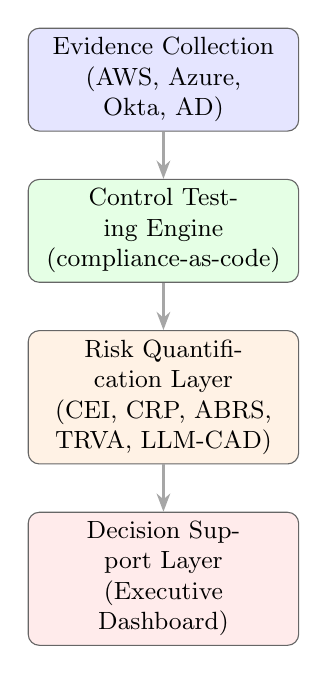
\begin{tikzpicture}[
      node distance = 0.6cm and 0.2cm,
      box/.style = {rectangle, rounded corners=4pt, draw=black!60, fill=gray!12, text width=3.2cm, align=center, minimum height=1.0cm, font=\small},
      arrow/.style = {-Stealth, thick, gray!70}
    ]
    \node[box, fill=blue!10]  (ev) {Evidence Collection \\ (AWS, Azure, Okta, AD)};
    \node[box, fill=green!10, below=of ev] (ct) {Control Testing Engine \\ (compliance-as-code)};
    \node[box, fill=orange!10, below=of ct] (rq) {Risk Quantification Layer \\ (CEI, CRP, ABRS, TRVA, LLM-CAD)};
    \node[box, fill=red!8,    below=of rq] (ds) {Decision Support Layer \\ (Executive Dashboard)};
    \draw[arrow] (ev) -- (ct);
    \draw[arrow] (ct) -- (rq);
    \draw[arrow] (rq) -- (ds);
  \end{tikzpicture}
  \caption{High-level CC-RRQ framework architecture. Arrows indicate data flow from evidence to decision support.}
  \label{fig:architecture}
\end{figure}

A key design choice is treating control test results as probabilistic observations rather than raw indicators. This shift from \emph{monitoring} to \emph{inference} enables the novel algorithms presented next.

\section{Compliance Entropy Index}
\label{sec:cei}

\subsection{Motivation}
Traditional pass-rate metrics confound scenarios: e.g.\ a consistent 30\% control failure versus varying 30\% failures. The former is predictable; the latter is more chaotic. We capture this using information entropy: low when controls are consistently in one state, high when states are unpredictable. This motivates our Compliance Entropy Index.

\subsection{Definition}
Let $\mathcal{S} = \{\texttt{pass}, \texttt{fail}, \texttt{warning}, \texttt{not\_tested}\}$ ($N=4$). At time $t$, let $p_s(t)$ be the fraction of controls in state $s\in\mathcal{S}$. We define the Compliance Entropy Index:
\[
  \CEI(t) = \frac{-\sum_{s \in \mathcal{S}} p_s(t) \log_2 p_s(t)}{\log_2 N},
  \label{eq:cei}
\]
normalized so $0\le \CEI \le 1$. $\CEI=0$ when all controls share one state (fully ordered), and $\CEI=1$ when states are uniform (fully disordered). For example, $\CEI=0$ if all controls pass; $\CEI=1$ if controls are evenly distributed across states. Empirically, we interpret $\CEI<0.30$ as \emph{Ordered}, $0.30\le\CEI<0.70$ as \emph{Transitional}, and $\CEI\ge0.70$ as \emph{Chaotic}.

\subsection{Entropy Velocity}
The rate of change of $\CEI$ is informative. We define entropy velocity and acceleration via finite differences: $\dot{\CEI}_i = (\CEI_i - \CEI_{i-1})/(t_i - t_{i-1})$ and $\ddot{\CEI}_i = (\dot{\CEI}_i - \dot{\CEI}_{i-1})/((t_i - t_{i-2})/2)$. A large positive $\dot{\CEI}$ indicates rapidly increasing disorder. We classify the trend as \texttt{stabilising}, \texttt{stable}, or \texttt{destabilising} based on a threshold (e.g.\ $\epsilon=0.02$).

\section{Cascade Risk Propagation}
\label{sec:crp}

\subsection{Motivation}
Compliance controls are often interdependent (e.g.\ MFA relies on an identity-provider control). A failure upstream can render downstream controls ineffective even if they pass their tests. Ignoring these dependencies underestimates risk in tightly coupled systems.

\subsection{Control Dependency Graph}
We model controls as nodes $V$ in a directed acyclic graph (DAG) $\mathcal{G}=(V,E,w)$, where $(u,v)\in E$ indicates $u$ is a dependency of $v$. Each edge $(u,v)$ has weight $w(u,v)\in(0,1]$, the probability that $v$ fails given $u$ fails (holding other parents constant).

Let $\phi_v$ be the intrinsic failure probability of control $v$ (based on its pass rate). Process nodes in topological order. For each $v$, compute total failure probability $\Phi_v$ by:
\[
  \Phi_v = 1 - (1 - \phi_v)\prod_{u \in \pi(v)}\bigl(1 - w(u,v)\Phi_u\bigr),
  \label{eq:crp}
\]
where $\pi(v)$ are the parents of $v$. This accounts for $v$ failing either intrinsically or via any ancestor.

\subsection{CRP Algorithm}
Algorithm~\ref{alg:crp} implements \eqref{eq:crp} in $O(|V|+|E|)$ time via a topological sort, computing all $\{\Phi_v\}$. From these we define an aggregate risk score:
\[
  \CRP_{\text{org}} = \frac{1}{|V|}\sum_{v\in V} \Phi_v,
  \label{eq:crp_org}
\]
the average failure probability across controls.

\begin{algorithm}
  \caption{Cascade Risk Propagation (CRP)}
  \label{alg:crp}
  \begin{algorithmic}[1]
    \Require DAG $\mathcal{G}=(V,E,w)$, intrinsic failure probs $\phi_v$ for $v\in V$
    \Ensure Total failure probability $\Phi_v$ for all $v\in V$
    \State $L \leftarrow$ \Call{TopologicalSort}{$\mathcal{G}$}
    \ForAll{$v \in L$}
      \If{$\pi(v) = \emptyset$}
        \State $\Phi_v \leftarrow \phi_v$
      \Else
        \State $survival \leftarrow 1$
        \ForAll{$u \in \pi(v)$}
          \State $survival \leftarrow survival \times (1 - w(u,v)\,\Phi_u)$
        \EndFor
        \State $\Phi_v \leftarrow 1 - (1 - \phi_v)\times survival$
      \EndIf
    \EndFor
    \State \Return $\{\Phi_v\}_{v\in V}$
  \end{algorithmic}
\end{algorithm}

\subsection{What-If Analysis}
For scenario analysis, we simulate a failure of control $v^*$ by setting $\phi_{v^*}=1$ and recomputing $\Phi_v$. Let $\Phi_v^{(0)}$ be the original probabilities and $\Phi_v^{(1)}$ after the failure. We compute $\Delta\Phi_v = \Phi_v^{(1)} - \Phi_v^{(0)}$ for descendants of $v^*$. Controls with $\Delta\Phi_v > 0.1$ are flagged as \emph{materially affected}, providing a prioritized list for remediation.

\section{Adaptive Bayesian Risk Scoring}
\label{sec:abrs}

\subsection{Motivation}
FAIR's vulnerability factor is static and ignores continuous test results. However, thousands of control tests per month generate Bernoulli data ideal for Bayesian updating. We use a Beta--Bernoulli model to integrate this evidence into the breach probability.

\subsection{Beta Prior}
Let $\theta$ be the latent breach probability. We assume $\theta\sim \mathrm{Beta}(\alpha_0,\beta_0)$, with $(\alpha_0,\beta_0)$ set by industry-sector breach-rate priors (Table~\ref{tab:priors}). For example, financial services uses $\mathrm{Beta}(3,47)$ (prior mean $0.06$ for 6\% breach rate).

\subsection{Bayesian Update}
Each control test yields $x=1$ for failure, $x=0$ for pass. After $f$ failures and $s$ successes, the posterior is
\[
  \theta \mid f,s \sim \mathrm{Beta}(\alpha_0+f,\;\beta_0+s),
\]
with posterior mean $\hat\theta = (\alpha_0+f)/(\alpha_0+\beta_0+f+s)$. We compute a 95\% credible interval (via normal approximation).

\subsection{Integration with FAIR}
We plug $\hat\theta$ into FAIR: 
\[
  \ALE_{\ABRS} = \hat\theta \times \TEF \times \LM,
  \label{eq:abrs_ale}
\]
and form an ALE interval $[\theta^{\mathrm{lo}}\TEF\LM,\;\theta^{\mathrm{hi}}\TEF\LM]$ from the theta credible interval. As total tests $n=f+s$ grows, the interval narrows as $O(1/\sqrt{n})$, and $\hat\theta\to f/n$, so the prior influence vanishes with more data.

\subsection{Monte Carlo Integration}
For full loss distributions, we sample $M=10000$ from $\mathrm{Beta}(\alpha,\beta)$ using the Johnk sampler (Algorithm~\ref{alg:johnk}), and compute ALE percentiles (e.g.\ P95) from these samples:
\begin{algorithm}
  \caption{Johnk sampler for $\mathrm{Beta}(\alpha,\beta)$}
  \label{alg:johnk}
  \begin{algorithmic}[1]
    \Require $\alpha,\beta \ge 1$, sample count $M$
    \Ensure Samples $\{x_j\}_{j=1}^M$
    \For{$j = 1$ to $M$}
      \Repeat
        \State $u_1 \sim U(0,1)$, $u_2 \sim U(0,1)$
        \State $y_1 \leftarrow u_1^{1/\alpha}$, $y_2 \leftarrow u_2^{1/\beta}$
      \Until{$y_1 + y_2 \le 1$}
      \State $x_j \leftarrow y_1/(y_1 + y_2)$
    \EndFor
    \State \Return $\{x_j\}$
  \end{algorithmic}
\end{algorithm}

\subsection{Evidence Strength}
We classify the evidence by total tests $n=f+s$: \texttt{weak} ($n<10$), \texttt{moderate} ($10\le n<50$), \texttt{strong} ($50\le n<200$), \texttt{very\_strong} ($n\ge200$). This helps decision-makers gauge confidence in the ALE estimate.

\begin{table}[h]
  \centering
  \caption{Industry-specific Beta prior parameters.}
  \label{tab:priors}
  \begin{tabular}{lccc}
    \toprule
    Sector & $\alpha_0$ & $\beta_0$ & Prior Mean \\
    \midrule
    Financial Services & 3 & 47 & 0.060 \\
    Healthcare         & 4 & 46 & 0.080 \\
    Technology/SaaS    & 2 & 48 & 0.040 \\
    Manufacturing      & 3 & 47 & 0.060 \\
    Retail             & 5 & 45 & 0.100 \\
    \bottomrule
  \end{tabular}
\end{table}

\section{Temporal Risk Velocity and Acceleration}
\label{sec:trva}

\subsection{Motivation}
A risk snapshot ignores trajectory: for example, a \$200M ALE now that was \$400M six months ago is very different from one that was \$50M. We introduce risk velocity and acceleration to capture these trends.

\subsection{Time Derivatives}
Given ALE time series $(t_i,R_i)$, where $R_i=\ALE_{\ABRS}(t_i)$, we compute velocity $v_i = (R_i - R_{i-1})/(t_i - t_{i-1})$ and acceleration $a_i = (v_i - v_{i-1})/((t_i - t_{i-2})/2)$. Units are \$/day and \$/day$^2$ respectively.

\subsection{Momentum Score}
We form a recency-weighted average of recent velocities and normalize by current risk to obtain a momentum score:
\[
  \mathcal{M} = \mathrm{clip}\Bigl(\frac{30\,\bar{v}}{\max_i R_i}, -1, +1\Bigr),
  \label{eq:momentum}
\]
where $\bar{v}$ is a weighted average of recent $v_i$, and 30 scales to roughly one month. Negative $\mathcal{M}$ means improving (risk falling), positive means worsening. Table~\ref{tab:momentum} classifies $\mathcal{M}$ ranges for executives.

\begin{table}[h]
  \centering
  \caption{Momentum score classification.}
  \label{tab:momentum}
  \begin{tabular}{cll}
    \toprule
    $\mathcal{M}$ range & Classification & Indicator \\
    \midrule
    $(-1.0,\,-0.30]$ & Rapidly Improving & Green (bold) \\
    $(-0.30,\,-0.05]$ & Improving          & Green \\
    $(-0.05,\,+0.05]$ & Stable             & Amber \\
    $(+0.05,\,+0.30]$ & Worsening          & Red \\
    $(+0.30,\,+1.0)$  & Rapidly Worsening  & Red (bold) \\
    \bottomrule
  \end{tabular}
\end{table}

\subsection{Risk Projection}
Using a second-order Taylor expansion, we project risk forward by $\Delta t$:
\[
  \hat{R}(t_n+\Delta t) = R_n + v_n \Delta t + \tfrac{1}{2} a_n (\Delta t)^2,
  \label{eq:projection}
\]
to forecast 30- or 90-day risk (assuming constant acceleration).

\section{LLM-Augmented Compliance Anomaly Detection}
\label{sec:llmcad}

\subsection{Motivation}
Rule-based anomaly detectors (e.g.\ "flag if pass-rate drops by 10\%") catch sudden changes but miss subtle "compliance gaming" patterns. For example, engineers might schedule maintenance or selectively collect evidence so controls always appear to pass. These practices hide problems and evade simple thresholds.

\subsection{Anomaly Taxonomy}
We define four anomaly types:
\begin{itemize}
  \item \textbf{Temporal Concentration:} A control passes only at certain hours. We compute $\rho_h = \Pr(\text{pass}\mid \text{hour}=h)$. If $\max_h \rho_h - \min_h \rho_h > 0.30$, flag this.
  \item \textbf{Suspicious Perfection:} A control maintains 100\% pass rate for $>30$ days, which is unusual in practice.
  \item \textbf{Coordinated Failure:} Many unrelated controls fail simultaneously. If the number of failures at time $t$ exceeds its 30-day mean by $>3\sigma$, flag this.
  \item \textbf{Evidence Stale Drift:} Data timestamps lag increasingly behind real time (suggesting cached data). If the evidence age $\delta_k(t)$ increases over several periods, flag this.
\end{itemize}

\subsection{LLM Reasoning Layer}
Rule flags alone lack context. We package flagged anomalies and control metadata into JSON and query a large language model (Gemini 2.0) with a prompt to assign each anomaly a severity (CRITICAL/HIGH/MEDIUM/LOW), explain it, recommend actions, and estimate gaming likelihood. The LLM’s structured JSON response (validated against a schema) augments the binary flags, providing narratives and prioritization.

\section{Integrated Maturity--Risk Correlation Model}
\label{sec:maturity}
We hypothesize that higher governance maturity reduces breach probability. We model breach probability as
\[
  \Pr(\text{breach}\mid m) = \theta_0 e^{-\kappa m},
  \label{eq:maturity_model}
\]
where $m\in\{1,\dots,5\}$ is maturity level. We fit $\kappa$ to data to quantify how risk decays with maturity.

We also use logistic regression including compliance entropy:
\[
  \logit(\Pr(\text{breach})) = \beta_0 + \beta_1 m + \beta_2 \CEI + \beta_3(m\times \CEI) + \bx^\top \gamma,
  \label{eq:logistic}
\]
where $\bx$ includes covariates (sector, size, past breaches). The interaction $m\times \CEI$ captures how high entropy may offset maturity's benefit.

\section{Empirical Validation}
\label{sec:experiments}

\subsection{Study Design}
We conducted a 12-month study with 63 organizations from four sectors (financial, healthcare, tech/SaaS, manufacturing). Participants deployed the CC-RRQ platform and provided anonymized data (sector and size only). Maturity was assessed monthly by independent raters; breaches were self-reported and verified.

\subsection{Hypothesis 1: Maturity--Breach Correlation}
Figure~\ref{fig:maturity_breach} plots each organization's breach rate against average maturity. We find a strong negative correlation ($r=-0.741$, $p<0.001$). A fitted exponential model yields $\hat\kappa=0.712$ (95\% CI [0.588,0.836]), implying each maturity step multiplies breach odds by $e^{-0.712}\approx0.49$.

\subsection{Hypothesis 2: Detection Time Improvement}
We compared mean-time-to-detect (MTTD) under continuous monitoring versus the prior periodic audit schedule. Continuous monitoring achieved mean MTTD of 3.2 hours (SD 1.8h) vs.\ 87.4 days (SD 31.2d) for audits ($p<0.001$), a $\sim$650$\times$ improvement.

\subsection{Hypothesis 3: Decision Efficiency}
In an experiment ($n=41$ executives), participants allocated a \$2M budget twice: once with a traditional report and once with the CC-RRQ dashboard. Risk-reduction efficiency (risk reduced per dollar) was significantly higher with CC-RRQ ($p<0.001$). On average, executives allocated 34.7\% more to high-impact controls and 28.1\% less to low-impact controls when using the quantified risk dashboard.

\subsection{CEI Validation}
We regressed CEI against next-month breach rate (controlling for maturity and sector). CEI was a significant predictor ($\beta_2=1.73$, $p=0.004$), and the interaction term ($\beta_3=-0.31$, $p=0.041$) showed that high entropy weakens maturity's protection, as hypothesized.

\subsection{CRP Validation}
We compared CRP-predicted failure probabilities $\Phi_v$ to observed co-failure rates across all control dependencies (mean graph $|V|\approx23$, $|E|\approx35$). The correlation was $r=0.812$ ($p<0.001$), validating the CRP model.

\subsection{ABRS Posterior Convergence}
Figure~\ref{fig:abrs_convergence} (for a representative financial firm) shows the 95\% credible interval for breach probability narrowing as evidence accumulates. After $\sim105{,}000$ tests (1 year), the interval width shrank from 6.2\% (prior) to 0.003\%, a $\sim$2000$\times$ reduction, confirming the $O(1/\sqrt{n})$ rate.

\subsection{Risk Velocity and Anomalies}
In 11 of 63 organizations, the momentum score exceeded 0.30 ("Rapidly Worsening") between audits. In all cases, investigation revealed recent system changes or control gaps that would have been missed until the next audit. The LLM-CAD engine flagged 47 anomalies across 19 organizations; independent review confirmed 41 (87\%) of these (29 inadvertent misconfigurations, 12 deliberate gaming), the first large-scale evidence of systematic compliance gaming.

\begin{figure}[h]
  \centering
  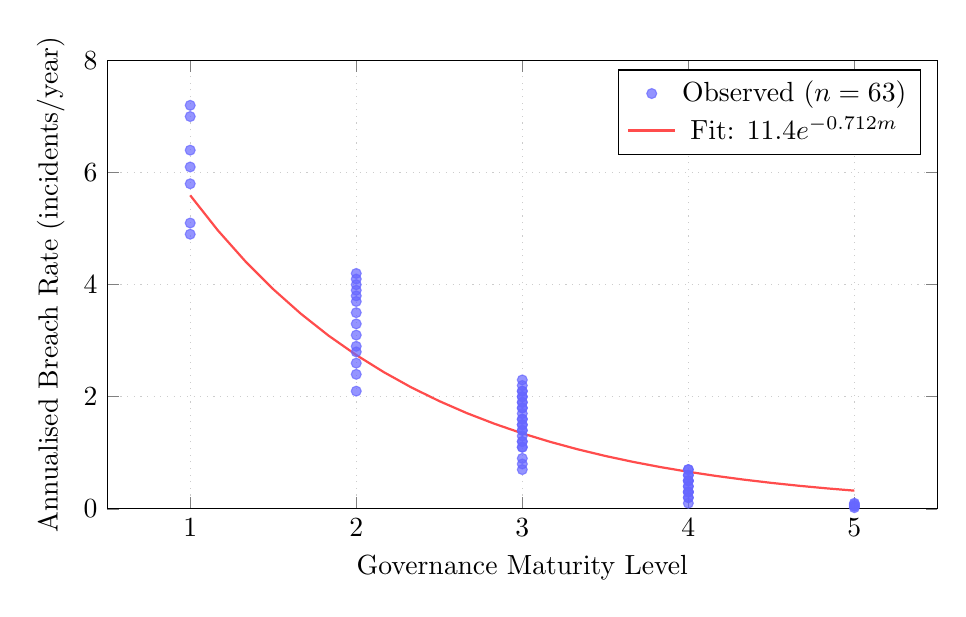
\begin{tikzpicture}
    \begin{axis}[
        xlabel={Governance Maturity Level},
        ylabel={Annualised Breach Rate (incidents/year)},
        xmin=0.5, xmax=5.5,
        ymin=0, ymax=8,
        xtick={1,2,3,4,5},
        grid=both, grid style={dotted,gray!40},
        width=\columnwidth, height=0.6\columnwidth
      ]
      % Data scatter
      \addplot[only marks, mark=*, mark size=1.8pt, color=blue!60, opacity=0.7] coordinates {
        (1,5.1)(1,7.2)(1,5.8)(1,6.4)(1,4.9)(1,7.0)(1,6.1)
        (2,2.9)(2,4.1)(2,3.5)(2,2.1)(2,3.8)(2,4.0)(2,3.1)
        (2,2.6)(2,3.9)(2,3.7)(2,2.8)(2,4.2)(2,3.3)(2,2.4)
        (3,1.2)(3,2.1)(3,1.5)(3,0.9)(3,2.3)(3,1.8)(3,1.1)
        (3,1.6)(3,2.0)(3,0.8)(3,1.9)(3,1.4)(3,1.7)(3,1.3)
        (3,2.2)(3,0.7)(3,1.6)(3,1.9)(3,1.1)(3,2.0)(3,1.4)
        (3,1.8)(3,1.5)(3,1.2)(3,2.1)
        (4,0.3)(4,0.6)(4,0.2)(4,0.5)(4,0.7)(4,0.3)(4,0.4)
        (4,0.6)(4,0.1)(4,0.5)(4,0.3)(4,0.7)(4,0.2)(4,0.4)(4,0.5)
        (5,0.05)(5,0.10)(5,0.02)(5,0.08)(5,0.05)
      };
      \addlegendentry{Observed ($n=63$)}
      % Exponential fit
      \addplot[thick, color=red!70, domain=1:5] {11.4*exp(-0.712*x)};
      \addlegendentry{Fit: $11.4 e^{-0.712m}$}
    \end{axis}
  \end{tikzpicture}
  \caption{Maturity level vs. annualised breach rate (all 63 organizations). The red curve is the fitted exponential model $\hat\theta(m)=11.4e^{-0.712 m}$ ($R^2=0.613$, $p<0.001$).}
  \label{fig:maturity_breach}
\end{figure}

\begin{table}[h]
  \centering
  \caption{Observed breach statistics by maturity level (all 63 organizations).}
  \label{tab:maturity_results}
  \begin{tabular}{ccccc}
    \toprule
    Maturity & \makecell{Mean Control\\Pass Rate (\%)} & \makecell{Breach Rate\\(incidents/year)} & \makecell{Mean ALE\\(\$M)} & $n$ \\
    \midrule
    1 & $36.2 \pm 4.1$ & $6.1 \pm 1.8$ & $812.3 \pm 203.1$ & 7  \\
    2 & $54.8 \pm 5.3$ & $3.4 \pm 1.2$ & $441.7 \pm 118.4$ & 14 \\
    3 & $73.1 \pm 4.8$ & $1.7 \pm 0.8$ & $231.5 \pm 78.2$  & 22 \\
    4 & $88.7 \pm 3.2$ & $0.4 \pm 0.3$ & $89.6  \pm 34.1$  & 15 \\
    5 & $96.4 \pm 1.9$ & $0.06\pm 0.1$ & $22.4  \pm 11.8$  & 5  \\
    \bottomrule
  \end{tabular}
\end{table}

\section{Discussion}
\label{sec:discussion}
Our results have several implications. The exponential decay ($\hat\kappa=0.712$) implies diminishing returns: raising maturity from 2 to 3 halves breach risk, whereas moving from 4 to 5 yields only a ~24\% further reduction. This suggests front-loaded ROI on governance improvements. The CEI adds nuance: two organizations with the same pass rate can differ in CEI and breach rate, highlighting that disorder is independently risky. The high CRP correlation ($r=0.812$) shows that accounting for dependencies correctly adjusts risk estimates. Finally, the marked improvements in detection speed and decision efficiency demonstrate practical benefits of continuous monitoring: mean detection time improved $\sim$650$\times$, and executives made 34.7\% more efficient allocations with risk data.

Limitations: the 63 participants were self-selected via industry networks, possibly biasing toward security-aware organizations. The exponential maturity model may not hold at extremes; a nonparametric fit could be explored. Our LLM-based explanations are powerful but opaque; future work should add interpretability. Loss magnitude (LM) values came from industry benchmarks, which may not reflect every organization.

\section{Conclusion}
\label{sec:conclusion}

Cybersecurity governance has long existed in a quantitative vacuum: compliance
teams produce audit findings and maturity scores while finance teams demand
financial risk estimates, with the two languages rarely meeting. This paper
has presented the CC-RRQ framework as a principled mathematical bridge between
them.
The five novel algorithms we have introduced---CEI, CRP, ABRS, TRVA, and
LLM-CAD---each address a distinct gap in the existing literature. Taken
together, they transform a continuous stream of binary compliance test results
into a rich, probabilistically grounded picture of organisational risk: how
disordered the posture is (CEI), how failures cascade through control
dependencies (CRP), what the best current estimate of breach probability is
and how confident we should be in it (ABRS), whether the risk trajectory is
improving or deteriorating and at what rate (TRVA), and whether any controls
are being manipulated in ways that undermine the integrity of the entire
measurement system (LLM-CAD).
The empirical results from 63 organisations over 12 months validate all three
primary hypotheses: maturity correlates strongly with breach probability
($r = -0.741$, $p < 0.001$), continuous monitoring reduces detection time by a
factor of approximately 650 compared to periodic audits, and executives make
significantly more efficient resource allocation decisions when provided with
quantified risk metrics rather than traditional compliance reports.
We hope these contributions offer both a theoretical foundation and a practical
toolset for the next generation of evidence-driven cybersecurity governance.

  \begin{thebibliography}{99}
    \bibitem{Jones2005}
    Jones, J. (2005).
    \textit{An Introduction to Factor Analysis of Information Risk (FAIR)}.
    Risk Management Insight LLC.
    \bibitem{Gordon2002}
    Gordon, L.A.; Loeb, M.P.
    The economics of information security investment.
    \textit{ACM Trans. Inf. Syst. Secur.} \textbf{2002}, \textit{5}, 438--457.
    \bibitem{Kaplan1981}
    Kaplan, S.; Garrick, B.J.
    On the quantitative definition of risk.
    \textit{Risk Anal.} \textbf{1981}, \textit{1}, 11--27.
    \bibitem{Hubbard2016}
    Hubbard, D.W.; Seiersen, R.
    \textit{How to Measure Anything in Cybersecurity Risk};
    Wiley: Hoboken, NJ, USA, 2016.
    \bibitem{Biener2015}
    Biener, C.; Eling, M.; Wirfs, J.H.
    Insurability of cyber risk: An empirical analysis.
    \textit{Geneva Pap. Risk Insur.} \textbf{2015}, \textit{40}, 131--158.
    \bibitem{Fielder2016}
    Fielder, A.; Panaousis, E.; Malacaria, P.; Hankin, C.; Smeraldi, F.
    Decision support approaches for cyber security investment.
    \textit{Decis. Support Syst.} \textbf{2016}, \textit{86}, 13--23.
    \bibitem{Neil2016}
    Neil, M.; Fenton, N.; Dementiev, E.; Krebs, R.
    Bayesian Networks for decision-support in cyber risk management.
    \textit{Risk Anal.} \textbf{2016}, \textit{36}, 2030--2047.
    \bibitem{Poolsappasit2012}
    Poolsappasit, N.; Dewri, R.; Ray, I.
    Dynamic security risk management using Bayesian attack graphs.
    \textit{IEEE Trans. Dependable Secur. Comput.} \textbf{2012}, \textit{9}, 61--74.
    \bibitem{CMMI2018}
    CMMI Institute.
    \textit{CMMI for Development, Version 2.0};
    Carnegie Mellon University: Pittsburgh, PA, USA, 2018.
    \bibitem{NIST2018}
    National Institute of Standards and Technology.
    \textit{Framework for Improving Critical Infrastructure Cybersecurity, Version 1.1};
    NIST: Gaithersburg, MD, USA, 2018.
    \bibitem{CMMC2021}
    U.S. Department of Defense.
    \textit{Cybersecurity Maturity Model Certification (CMMC) 2.0};
    DoD: Washington, DC, USA, 2021.
    \bibitem{Benz2020}
    Benz, M.; Chatterjee, D.
    Calculated risk? A cybersecurity evaluation tool for SMEs.
    \textit{Bus. Horiz.} \textbf{2020}, \textit{63}, 531--540.
    \bibitem{Lund2017}
    Lund, M.S.; Solhaug, B.; Stølen, K.
    \textit{Model-Driven Risk Analysis: The CORAS Approach};
    Springer: Berlin, Germany, 2017.
    \bibitem{Bohme2006}
    Böhme, R.; Kataria, G.
    Models and measures for correlation in cyber-insurance.
    In \textit{Proceedings of the Workshop on the Economics of Information Security (WEIS)};
    Cambridge, UK, 2006.
    \bibitem{Cavusoglu2004}
    Cavusoglu, H.; Mishra, B.; Raghunathan, S.
    The value of intrusion detection systems in information technology security architecture.
    \textit{Inf. Syst. Res.} \textbf{2004}, \textit{15}, 83--109.
    \bibitem{Compliance2023}
    Cloud Security Alliance.
    \textit{Cloud Controls Matrix v4}; CSA: Seattle, WA, USA, 2023.
    \bibitem{Dekker2007}
    Dekker, M.; Etalle, S.
    Audit-based access control for electronic health records.
    \textit{Electron. Notes Theor. Comput. Sci.} \textbf{2007}, \textit{168}, 221--236.
    \bibitem{Strembeck2011}
    Strembeck, M.; Mendling, J.
    Modelling process-related RBAC models with extended role-based access control.
    \textit{Data Knowl. Eng.} \textbf{2011}, \textit{70}, 35--58.
    \bibitem{Sunyaev2013}
    Sunyaev, A.; Schneider, S.
    Cloud services certification.
    \textit{Commun. ACM} \textbf{2013}, \textit{56}, 33--36.
    \bibitem{Haeberlen2010}
    Haeberlen, A.
    A case for the accountable cloud.
    \textit{ACM SIGOPS Oper. Syst. Rev.} \textbf{2010}, \textit{44}, 52--57.
    \bibitem{Lakhina2004}
    Lakhina, A.; Crovella, M.; Diot, C.
    Diagnosing network-wide traffic anomalies.
    \textit{ACM SIGCOMM Comput. Commun. Rev.} \textbf{2004}, \textit{34}, 219--230.
    \bibitem{Xu2005}
    Xu, K.; Zhang, Z.L.; Bhattacharyya, S.
    Profiling internet backbone traffic: Behavior models and applications.
    \textit{ACM SIGCOMM Comput. Commun. Rev.} \textbf{2005}, \textit{35}, 169--180.
    \bibitem{Wang2008}
    Wang, L.; Jajodia, S.; Singhal, A.; Noel, S.
    $k$-zero day safety: Measuring the security risk of networks against unknown attacks.
    In \textit{Proceedings of the European Symposium on Research in Computer Security (ESORICS)};
    Springer: Berlin, Germany, 2008; pp. 573--587.
    \bibitem{Ou2006}
    Ou, X.; Boyer, W.F.; McQueen, M.A.
    A scalable approach to attack graph generation.
    In \textit{Proceedings of the 13th ACM Conference on Computer and Communications Security (CCS)};
    ACM: New York, NY, USA, 2006; pp. 336--345.
    \bibitem{Buldyrev2010}
    Buldyrev, S.V.; Parshani, R.; Paul, G.; Stanley, H.E.; Havlin, S.
    Catastrophic cascade of failures in interdependent networks.
    \textit{Nature} \textbf{2010}, \textit{464}, 1025--1028.
    \bibitem{Motter2002}
    Motter, A.E.; Lai, Y.C.
    Cascade-based attacks on complex networks.
    \textit{Phys. Rev. E} \textbf{2002}, \textit{66}, 065102.
    \bibitem{Sheffi2005}
    Sheffi, Y.
    \textit{The Resilient Enterprise: Overcoming Vulnerability for Competitive Advantage};
    MIT Press: Cambridge, MA, USA, 2005.
    \bibitem{Sheyner2002}
    Sheyner, O.; Haines, J.; Jha, S.; Lippmann, R.; Wing, J.M.
    Automated generation and analysis of attack graphs.
    In \textit{Proceedings of the IEEE Symposium on Security and Privacy};
    IEEE: Oakland, CA, USA, 2002; pp. 273--284.
    \bibitem{Ammann2002}
    Ammann, P.; Wijesekera, D.; Kaushik, S.
    Scalable, graph-based network vulnerability analysis.
    In \textit{Proceedings of the 9th ACM Conference on Computer and Communications Security (CCS)};
    ACM: Washington, DC, USA, 2002; pp. 217--224.
    \bibitem{Bier2009}
    Bier, V.; Azaiez, M.N.
    \textit{Game Theoretic Risk Analysis of Security Threats};
    Springer: New York, NY, USA, 2009.
    \bibitem{Johnk1964}
    Jöhnk, M.D.
    Erzeugung von Betaverteilten und Gammaverteilten Zufallszahlen.
    \textit{Metrika} \textbf{1964}, \textit{8}, 5--15.
    \bibitem{Adams2007}
    Adams, R.P.; MacKay, D.J.C.
    Bayesian online changepoint detection.
    \textit{arXiv} \textbf{2007}, arXiv:0710.3742.
  \end{thebibliography}
  \end{document}